\newpage
%\section*{Summary}


\section{Decision theory\label{sec:decision}}
%Decision theory is re-developed. How should an individual decide whether to take some gamble (the usual way of phrasing decision problems in economics)? We solve typical decision problems (gamble evaluation) by considering the time-average growth rate (or the [time- and ensemble-] average of the ergodic growth rate) under multiplicative dynamics. The construction of an ergodic observable motivates the introduction of a non-linear function that encodes the dynamics. This function is historically called the “utility function” and encodes the dynamics. 
%
%In life we frequently find ourselves in situations which require us to make decisions, \ie to choose between two or more available actions whose outcomes may be uncertain. In this lecture we shall develop a theory of how individuals make such decisions. Of course, this is far too broad a promise. We can't possibly develop a {\it complete} theory of decisions in a single lecture, and perhaps not even in a lifetime. Indeed, since we will be studying mathematical models of decisions, we will necessarily have little to say about actions whose outcomes cannot be quantified, \eg in pounds, shillings, and pence. This lecture will not tell you whom you should marry or even whose economics lectures you should attend.
%
%Instead, we will narrow our gaze to problems which are mathematically tractable but, we hope, no less illuminating for being so. Specifically we will solve the gamble problem, which is the canonical problem in decision theory. Its treatment forms the cornerstone on which much of classical economics -- such as utility theory, game theory, and asset pricing -- is built.

%We shall not consider whether our theory is prescriptive, in that it informs us how individuals {\it should} make decisions, or descriptive, in that informs us how they {\it do}. This is an important epistemological question in decision theory but, for now at least, we will leave it to the philosophers.

{\it Decision theory is a cornerstone of formal economics. As the name suggests, it 
models how people make decisions. In this chapter we will generalise and formalise
the treatment of the coin tossing game to introduce our 
approach to decision theory. Our central axiom will be that people attempt to maximize
the rate at which wealth grows when averaged over time. This is a surprisingly powerful idea.
In many cases it eliminates the need for well established but epistemologically troublesome techniques, such as utility functions. 
}
\newpage

\subsection{Models and science fiction}
We will do decision theory 
by using mathematical models, and since this can be done in many ways we will be
explicit about how we choose to do it. We will define a gamble, which 
is a mathematical object, and we will define a decision criterion. The gamble will be
reminiscent of real-world situations; and the decision criterion may or may not be reminiscent
of how real people make decisions. We will not worry too much about the accuracy 
of these reminiscences. Instead we will ``shut up and calculate'' -- we will let the mathematical
model create its world. Writing down a mathematical model is like laying out the premise for
a science-fiction novel. We may decide that people can download their consciousness onto a computer, 
that medicine has advanced to eliminate ageing and death -- these are premises we are at liberty to invent.
Once we have written them down we begin to explore the world that results from those premises.
A choice of decision criterion implies an endless list of behaviors that will
be observed. For example, some criteria will lead to cooperation, others will not, some will lead
to the existence of insurance contracts, others will not \etc We will explore the worlds created by the different
models. Once we have done so we invite you to judge which model may be more useful
for your understanding of the world. Of course, having spent many years thinking about these
issues we have come to our own conclusions, and we will put them forward because we believe them to be helpful.

To keep the discussion to a manageable volume we will only consider the gamble problem. 
This is reminiscent of making decisions in an uncertain context -- where we have to decide on
a course of action now although we don't know with certainty what will happen to us under any
of our choices. To limit the debate even further, we will only consider a setup that corresponds to
making purely financial decisions. We may bet on a horse or take out personal liability insurance.
This chapter will not tell you whom you should marry or even whose economics lectures you should attend.

%%%%%%%%%%%%%%%%%%%%%%%%%%%%%%%%%%%%%%%%%%%%%%%
\subsection{Gambles}
One fundamental building block of mathematical decision theory is the gamble.
This is a mathematical object that resembles a number of situations in real life, 
namely situations where we face a decision whose consequences will be purely
financial and are somewhat uncertain when we make the decision. A real-world example would be buying a lottery ticket. We define the gamble mathematically as follows.

\begin{defn}{Gamble}
A gamble is a pair of a random variable, $\gD$, and a duration,  $\dt$. 
\vspace{.2cm}

$\gD$ is called the payout and takes one of $\N$ (mutually exclusive) possible monetary 
values, 
$\{\gD_1,\ldots,\gD_N\}$, associated with probabilities, $\{\p_1,\ldots,\p_\N\}$, where 
$\sum_{\gi=1}^\N \p_\gi = 1$. 
Payouts can be positive, associated with a monetary gain, or negative, 
associated with a loss. We order them such that $\gD_1<\ldots<\gD_\N$.
\end{defn}

Everything we need to know about the gamble is contained in the 
payouts, probabilities, and duration.
We relate it to reality through a few examples:

\begin{example}{Betting on a fair coin}
Imagine betting $\$ 10$ on the toss of a fair coin. We would model this 
with the following payouts and probabilities:
\bea
\gD_1 = -\$ 10, &\quad& \p_1 = 1/2;\\
\gD_2 = +\$ 10, &\quad& \p_2 = 1/2.
\eea
The duration would be $\dt=2$ seconds.
\end{example}

\begin{example}{Playing the lottery}
We can also imagine a gamble akin to a lottery, where our individual pays an amount, 
$\F$, for a ticket which will win the jackpot, $\J$, with probability, $\p$. The corresponding 
payouts and probabilities are:
\bea
\gD_1 = -\F,  &\quad& \p_1 = 1-\p;\\
\gD_2 = \J-\F, &\quad& \p_2 = \p.
\eea
Note that we deduct the ticket price, $\F$, in the payout $\gD_2$.
The duration would be $\dt=1$ week.
\end{example}

\begin{example}{Betting at fixed odds}
A bet placed at fixed odds, for example on a horse race can also be modelled as a gamble. 
Suppose we bet on the horse \textit{Ito} to win the 2015 Prix de l'Arc de Triomphe 
in Paris at odds of 50/1 (the best available odds on 20th September 2015). 
\textit{Ito} will win the race with unknown probability, $\p$. If we bet $\F$, 
then this is modelled by payouts and probabilities:
\bea
\gD_1 = -\F,  &\quad& \p_1 = 1-\p;\\
\gD_2 = 50\F, &\quad& \p_2 = \p.
\eea
The duration would be something like $\dt=30$ minutes.
\end{example}

\begin{example}{The null gamble}
It is useful to introduce the null gamble, in which a payout of zero is received 
with certainty: $\gD_1=\$0$, $\p_1=1$. This represents the `no bet' or `do nothing' option.
The duration, $\dt$, has to be chosen appropriately. The meaning of the
duration will become clearer later on -- often it is the time between two successive rounds
of a gamble.
\end{example}

The gamble is a simple but versatile mathematical model of an uncertain future. 
It can be used to model not only traditional wagers, such as sports bets and 
lotteries, but also a wide range of economic activities, such as stock market 
investments, insurance contracts, derivatives, and so on. The gamble we have 
presented is discrete, in that the payout, $\gD$, is a random variable with a 
countable (and, we usually assume, small) number of possible outcomes. 
The extension to continuous random variables is natural and used frequently 
to model real-world scenarios where the number of possible outcomes, \eg the change 
in a stock price over one day, is large.

Suppose now that you have to choose between two options that you've modeled 
as two gambles (possibly including the null gamble). Which should you choose, 
and why? This is the gamble problem, the central question of decision theory, and 
the basis for much of mainstream economics.

%%%%%%%%%%%%%%%%%%%%%%%%%%%%%%%%%%%%%%%%%%%%%%%
\subsection{Repetition and wealth evolution}
To solve the gamble problem we must propose a criterion to choose between two
gambles. Different criteria will result in different decisions -- by writing down a criterion
we build a model world of model humans who behave in ways that may seem sensible
to us or crazy -- if the behavior seems crazy we have probably not chosen a good
criterion and we should try a different one.

The wealth process $\x(\t)$ is connected to the gambles our model humans 
choose to play. Precisely {\it how} it is affected remains to be specified.

Considering a single round of a gamble in isolation -- the so-called `one-shot 
game' of game theory -- is relatively uninstructive in this regard. All we know is 
that one of the possible payouts will be received, leading to the random variable 
$\x(\t+\dt)=\x(\t)+\gD$. 
We don't yet know how accepting this gamble will affect how our wealth, $\x(\t)$, grows or decays over time, since one time step isn't enough for this to become apparent. 
The one-shot game takes one random variable, $\gD$, and turns it trivially into 
another, $\x(\t)+\gD$. Time has no significance in a 
one-shot game. An amount $\dt$ elapses, but this could be a single 
heartbeat or the lifetime of the universe, for all the difference it makes to the analysis.

To establish how your wealth evolves, we must imagine that the world does 
not come to a grinding halt after the gamble. Instead we imagine that the gamble
is repeated over many rounds.\footnote{In fact, to make the 
problem tractable mathematically, it will be necessary to imagine the gamble 
is repeated indefinitely.} This does not mean that we actually
believe that a real-world situation will repeat itself over and over again, \eg we don't
believe that we will bet on the horse \textit{Ito} at odds 50/1 many times in a row. Instead, 
imagining repetition is a methodological device that allows us to extract tendencies
where they would otherwise be invisible. It is the model analogue of 
the idea that individuals live in time and that their decisions have consequences 
which unfold over time.

Crucially, {\it the mode of repetition is not specified in the gamble itself.} It is a 
second component of the model, which must be specified separately. Initially we shall 
focus on two modes: \textit{additive} and \textit{multiplicative} repetition. Other dynamics will be considered later on, in \secref{general_dynamics}.

\begin{defn}{Additive repetition}
If a gamble is repeated additively then  
the random payout, $\gD$, is simply added to $\x(\t)$ 
at each round. We define the change in wealth occurring 
over a single round as
\be
\d \x(\t) \equiv \x(\t+\dt)-\x(\t).
\elabel{DW_def}
\ee
In the additive case, we have
\be
\d\x(\t) = \gD.
\elabel{DW_add}
\ee
In other words, under additive repetition, $\d \x$ is a stationary 
random variable.
%\footnote{This seemingly mundane corollary stems 
%from our definitions of $\gD$ as a monetary payout and $\d\x$ as an 
%additive change in wealth, expressed in monetary units. It would not 
%hold if, for example, we had defined $\d\x$ to be some other type of 
%change, such as a relative change.}
Starting at time, $\tn$, wealth 
after $\T$ rounds is
\be
\x(\tn+\T\dt) = \x(\tn) + \sum_{\gtau=1}^\T \gD(\gtau),
\elabel{Wt_add}
\ee
where $\gD(\gtau)$ is the realisation of the random variable in round $\gtau$. 
This is an evolution equation for wealth following a noisy additive dynamic. 
Note that $\x(\tn+\T\dt)$ is itself a random variable.
\end{defn}


\begin{example}{Additive repetition}
We return to our first example of a gamble: a $\$ 10$ bet on 
a coin toss. Under additive repetition, successive bets will always 
be $\$ 10$, regardless of how rich or poor you 
become. Suppose your starting wealth is $\x(\tn)=\$ 100$. 
Then, following \eref{Wt_add}, your wealth after $\T$ rounds will be
\bea
\x(\tn+\T\dt) &=& \$ 100 + \$ 10 \gk - \$ 10 (\T-\gk)\\
&=& \$ [100 +  10(2\gk-\T)],
\eea
where $0\leq \gk\leq \T$ is the number of tosses you've won. Note that
we have assumed your wealth is allowed to go negative. If not, then the 
process would stop when $\x<\$ 10$, since you would be unable 
to place the next $\$ 10$ bet.
\end{example}

An alternative is multiplicative repetition. In the example above, let 
us imagine that the first $\$ 10$ bet were viewed not as a bet 
of fixed monetary size, but as a fixed fraction of the 
starting wealth ($\$ 100$). Under multiplicative repetition, each 
successive bet is for the same fraction of wealth which, 
in general, will be a different monetary amount.

The formalism is as follows. The payout, $\gD$, in the first round is 
expressed instead as a random wealth multiplier,
\be
\gr \equiv \frac{\x(\tn)+\gD}{\x(\tn)}.
\elabel{R_def}
\ee
The gamble is repeated by applying another realisation of the same multiplier at all subsequent rounds:
\be
\x(\t+\dt) = \gr\x(\t).
\ee
From \eref{R_def} we see that $\gr$ is a stationary random variable, 
since it depends only on $\gD$, which is stationary, and the starting 
wealth, $\x(\tn)$, which is fixed. However, successive changes in wealth,
\be
\d \x(\t) = (\gr-1)\x(\t),
\elabel{DW_mult_short}
\ee
are not stationary, as they depend on $\t$ through $\x(\t)$. The wealth 
after $\T$ rounds of the gamble is
\be
\x(\tn+\T\dt) = \x(\tn)\prod_{\gtau=1}^\T \gr(\gtau),
\ee
where $\gr(\gtau)$ is the realisation of the random multiplier in round $\gtau$.

\begin{example}{Multiplicative repetition}
The $\$10$ bet on a coin toss is now re-expressed as a bet of a fixed 
fraction of wealth at the start of each round. Following 
\eref{R_def}, the random multiplier, $\gr$, has two possible outcomes:
\bea
\gr_1 = \frac{\$100 - \$10}{\$100} = 0.9, &\quad& \p_1 = 1/2;\\
\gr_2 = \frac{\$100 + \$10}{\$100} = 1.1, &\quad& \p_2 = 1/2.
\eea
The wealth after $\T$ rounds is, therefore,
\be
\x(\tn+\T\dt) = \$100\,\,(1.1)^\gk\,(0.9)^{\T-\gk},
\ee
where $0\leq \gk \leq \T$ is the number of winning tosses. In this example there is 
no need to invoke a `no bankruptcy' condition, since our individual can lose no 
more than 10\% of his wealth in each round.
\end{example}

The difference between the two modes of repetition might easily be mistaken 
for a matter of taste. When the $\$ 10$ bet was first offered, what 
difference does it make whether our individual imagined this to be a bet of a 
fixed size or of a fixed fraction of his wealth? However, the consequences of 
this choice between imagined situations are enormous. As we saw in the 
previous lecture, additive and multiplicative dynamics differ as starkly as the 
linear and exponential functions. It matters, therefore, that we consider 
carefully the economic situation we wish to model in order to choose the 
most realistic mode of repetition. For example, fluctuations in the price of a 
stock tend to be proportional to the price, \cf \eref{DW_mult_short}, so 
multiplicativity is the appropriate paradigm here.

Now that we've established how the gamble is related to $\x(\t)$ we can 
begin to think about decision criteria. Not surprisingly, appropriate
growth rates are useful decision criteria -- ``pick the gamble that will lead
your wealth to grow the fastest'' is generally good advice. To be able to 
follow this advice we will think again about growth rates.

%%%%%%%%%%%%%%%%%%%%%%%%%%%%%%%%%%%%%%%%%%%%%%%
\subsection{Growth rates}
In the previous lecture we introduced the concept of a growth rate, $\g$, which 
is the rate of change of a monotonically increasing function of wealth, $\gv(\x(\t))$:
\be
\g(\t,\Dt) \equiv \frac{\D \gv(\x(\t))}{\Dt}.
\elabel{g_def}
\ee
The function, $\gv$, is chosen such that the increment, $\D \gv(\x(\t))$, over 
the period $\Dt$,\footnote{Note that we use a general time period, $\Dt$, here 
and not the period of the gamble, $\dt$.} is a stationary random variable 
whose distribution does not depend on when the period starts. The growth 
rate is, therefore, also stationary. Indeed, we consider it a function of $\t$ only 
inasmuch as this labels a particular realisation of the randomness at a particular point in time.

Stationarity -- the statistical irrelevance of the time of measurement -- is 
important because we want the distribution of the random growth rate 
to convey robust information about the underlying process, rather than 
mere happenstance about when it was sampled. 

%Therefore, the increments in any function $\gv(\x)$ will also be stationary. We want $\gv(\x)$ to be increasing in $\x$.
Under additive repetition, we know from \eref{DW_add} that $\D\x$ is already stationary, so we know immediately that the correct mapping is the identity: $\gv(\x)=\x$.\footnote{In fact, any linear function $\gv(\x)=\alpha\x+\beta$ has stationary increments and is monotonically increasing provided $\alpha>0$. However, there is nothing gained by choosing anything other $\gv(\x)=\x$.} This gives the growth rate for an additive process (denoted by the subscript `a'):
\be
\g_\text{a}(\t,\Dt) = \frac{\D\x(\t)}{\Dt}.
\elabel{g_add}
\ee

For a multiplicative dynamic, however, using $\d\x$ in the numerator 
of the rate will not do, as we know from \eref{DW_mult_short} that 
changes in $\x(\t)$ depend on $\x(\t)$. Instead we must find the 
mapping $\gv(\x)$ whose increment has a stationary distribution. 
The correct mapping is the logarithm, since the increment over a single round is
\bea
\d\ln \x(\t) &=& \ln \x(\t+\d\t) - \ln \x(\t)\\
&=& \ln \gr\x(\t) - \ln \x(\t)\\
&=& \ln \gr,
\eea
where \eref{R_def} has been used in the second line. This inherits its 
stationarity from $\gr$. Thus the appropriate growth rate for a multiplicative 
process (denoted by the subscript `m') over an arbitrary time period is
\be
\gm(\t,\Dt) = \frac{\D\ln \x(\t)}{\Dt}.
\elabel{g_mult}
\ee

The distribution of the stationary random variable 
$\g(\t,\Dt)$ depends on $\Dt$. Subject to certain conditions on $\D \gv(\x(\t))$, 
the distribution of $\g(\t,\Dt)$ narrows as $\Dt$ increases, converging to a 
finite number in the limit $\Dt\to\infty$. In other words, as the effect of the 
gamble manifests itself over an increasingly long time, the noise is eliminated 
to reveal a growth rate reflecting the gamble's underlying tendency.

We define this time-average growth rate, $\gt$, as
\be
\gt \equiv \lim_{\Dt\to\infty}\{\g(\t,\Dt)\}.
\ee
This is the growth rate that an individual will experience almost surely 
(\ie with probability approaching one) as the number of rounds of the 
gamble diverges. Indeed, we can express $\gt$ in precisely these terms,
\be
\gt = \lim_{\T\to\infty} \left\{ \frac{ \gv(\x(\t+\T\dt)) - \gv(\x(\t)) }{\T\dt } \right\},
\ee
where $\T$ is the number of rounds. Expanding the numerator as a sum 
of increments due to individual rounds of the gamble gives
\bea
\gt &=& \lim_{\T\to\infty} \left\{ \frac{1}{\T} \sum_{\gtau=1}^\T \frac{ \D \gv(\x(\t+\gtau\dt)) }{ \dt } \right\} \\
&=& \lim_{\T\to\infty} \left\{ \frac{1}{\T} \sum_{\gtau=1}^\T \g(\t+\gtau\dt,\dt) \right\} \\
&=& \ave{\g(\t,\dt)},
\eea
where the final line follows from the stationarity and independence of the successive 
per-round growth rates. This is a restatement of the ergodic property of the previous 
lecture, namely that the time-average growth rate can be expressed equivalently as 
the long-time limit and as the ensemble average of the properly chosen ergodic 
growth rate. For additive and multiplicative dynamics, we obtain the following 
equivalences:
\begin{align}
\gt_\text{a} &= \lim_{\Dt\to\infty}\left\{\frac{\D\x(\t)}{\Dt}\right\} = \ave{\frac{\D\x(\t)}{\Dt}}; \elabel{g_bar_a}\\
\gt_\text{m} &= \lim_{\Dt\to\infty}\left\{\frac{\D\ln \x(\t)}{\Dt}\right\} = \ave{\frac{\D\ln \x(\t)}{\Dt}}. \elabel{g_bar_m}
\end{align}
These follow the form of the general expression,
\be
\gt = \lim_{\Dt\to\infty}\left\{\frac{\D \gv(\x(\t))}{\Dt}\right\} = \ave{\frac{\D \gv(\x(\t))}{\Dt}}. \elabel{g_bar_gen}
\ee 
The value of $\Dt$ in the ensemble averages is immaterial. In calculations, 
it is often set to the period, $\dt$, of a single round of the gamble.

Where we are interested in the value of $\gt$, knowing that it is equal 
to the value of $\ave{\g}$ may provide a convenient method of calculating it. 
However, we will attach no special interpretation to the fact that $\ave{\g}$ is 
an expectation value. It is simply a quantity whose value happens to 
coincide with that of the quantity we're interested in, \ie the time-average 
growth rate.

Let's take a step back and remark more generally on what we have done so far. We 
started with a high-dimensional mathematical object, namely the 
probability distribution of the payout, $\gD$, of the gamble. To this we 
added two model components: the time period, $\dt$, over which the 
gamble unfolds; and a dynamic, in essence a set of instructions, specifying 
how the repeated gamble causes your wealth to evolve. We 
then collapsed all of this information into a single number, 
$\gt$, which characterises the effect of the gamble. The collapse from 
distribution to single number (or, equivalently, from uncertain to certain 
quantity) allows different gambles to be compared and, in particular, 
ranked. This permits an unequivocal decision criterion, which would be 
much harder to formulate for higher-dimensional objects, such as the 
two distributions shown in \fref{dec_dist}.
\begin{figure}
\centering
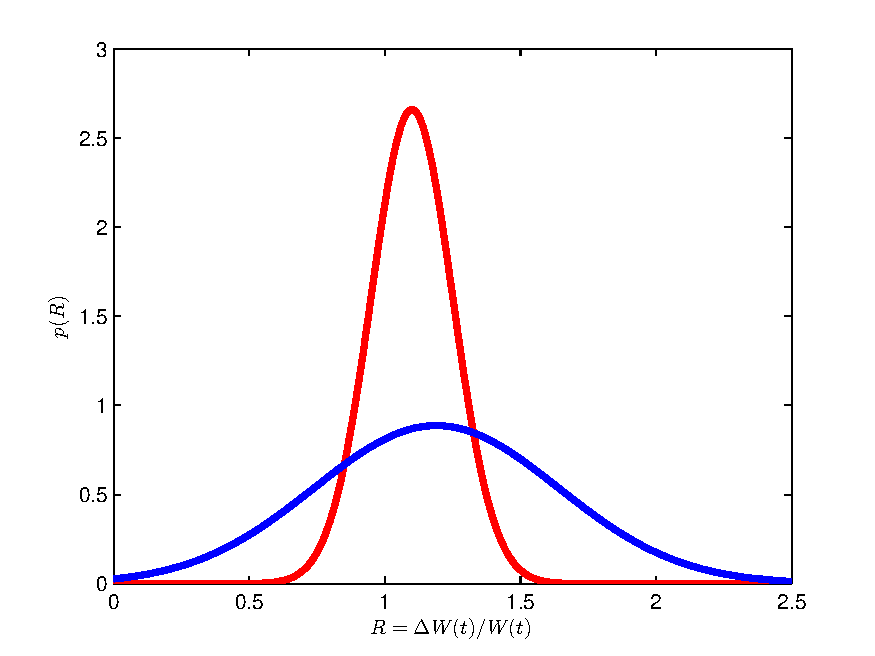
\includegraphics[width=0.9\textwidth]{./chapter_2/figs/dec_dist.pdf}
\caption{Two possible probability density functions for the per-round 
multiplier, $\gr$, defined in \eref{R_def}. The distribution denoted by 
the blue line has a higher mean and a higher variance than the one 
in red. How are we to decide which represents the more favourable 
gamble?\flabel{dec_dist}}
\end{figure}

%%%%%%%%%%%%%%%%%%%%%%%%%%%%%%%%%%%%%%%%%%%%%%%
\subsection{The decision axiom}
Our model rationale for deciding between two gambles is simple: 
given a model for the mode of repetition, 
choose the gamble with the largest time-average growth rate. 
In other words, choose the gamble which, 
if repeated indefinitely, causes your wealth to grow fastest.

We are not saying that real repetitions are necessary. We 
merely create model humans who base decisions on what would 
happen to their wealth if they were repeated (infinitely many times). It is a 
conceptual device -- in effect a thought experiment -- to elicit the 
underlying tendency of each gamble. A particular choice that can be 
represented by gambles 
may be offered only once and, indeed, in the real world this will 
often be the case. However, in the real world it is also the case 
that a decision is likely to be followed by many others, a scenario 
to which indefinite repetition is a plausible approximation.

In our thought experiment this decision rule outperforms any other 
decision rule almost surely: so, at least in that imagined world, the 
rationale has a logical basis. If our thought experiment is a good 
approximation to real-world decision scenarios, then our rationale 
should be a good model of real-world decisions. Certainly it is 
parsimonious, based on a single, 
robust quantity and requiring only the gamble and its mode of repetition 
to be specified. Unlike some treatments of human decision-making, it 
contains no arbitrary or hard-to-measure psychological factors.

Having said all this, while we think that the decision axiom 
is reasonable, we stress that it is an \textit{axiom}, \ie something we assert without empirical justification and which is not deduced from more primitive considerations. It 
defines a model world where certain types of behaviour will be observed. 
We feel reminded of reality by this model world, but you may disagree 
or you may prefer a different model that creates a different model world
that also reminds you of reality.
Other decision axioms are 
possible and, indeed, have been proposed. For instance, 
classical decision theory is defined by the axiom that decision
makers maximize expected utility. 

Our decision rationale can be expressed as a set of instructions.
We denote quantities relating to the $\m^\text{th}$ available gamble with the 
superscript $(\m)$. Each gamble is specified by its random payout, $\gD^{(\m)}$, and 
per-round period, $\dt^{(\m)}$. 

\begin{keypts}{Growth-optimal decision algorithm}
\begin{enumerate}
\item Specify $\gD^{(\m)}$ and $\dt^{(\m)}$ for the gambles offered;
\item Specify the wealth dynamic, \ie the relationship between $\d\x(\t)$, 
$\x(\t)$, and $\gD$;
\item Find the stationarity transformation, $\gv(\x)$, of the wealth whose increments are 
stationary random variables under this dynamic;
\item Determine the time-average growth rates, $\gt^{(\m)}$, either by taking 
the long-time limits of the growth rates, $\g^{(\m)}(\t,\dt)$, or by invoking the 
ergodic property to take their ensemble averages;
\item Choose the gamble, $\m$, with the largest time-average growth rate.
\end{enumerate}
\end{keypts}

In examples, we will focus on choices between two 
gambles, \ie $\m\in\{1,2\}$. Decisions between three or more gambles 
are straightforward extensions.
Often one of the gambles presented is the null gamble, which trivially 
has a growth rate of zero. In this case, the question then posed is 
whether the other gamble presented is preferable to doing nothing, 
\ie bet or no bet?

We will illustrate the decision algorithm by applying it to the coin toss 
game of the previous lecture. $\x(\tn)>\$ 0$ is the starting 
wealth and $\dt$ is the time between rounds for each of the 
gambles offered. We recall that the coin toss gamble is specified by the random payout:
\bea
\gD^{(1)}_1 = -0.4\x(\tn), &\quad& \p^{(1)}_1 = 1/2; \\
\gD^{(1)}_2 = 0.5\x(\tn), &\quad& \p^{(1)}_2 = 1/2.
\eea
Note that, in our setup, the payouts $\gD^{(\m)}_\gi$ are always fixed 
monetary amounts. Here they are expressed as fractions of $\x(\tn)$, 
which is itself a fixed monetary wealth.\footnote{Even though this 
formulation might appear to encode a multiplicative dynamic (largely 
because it comes from an imagined multiplicative game), we have 
arranged things so that formally it does not. Indeed, it encodes no 
dynamic at all: that is specified separately.} We shall ask our individual 
to choose between the coin toss and the null gamble,
\be
\gD^{(2)}_1 = \$0, \quad \p^{(2)}_1 = 1.
\ee
Both the additive and multiplicative versions of the repeated gamble are analysed.

\begin{example}{Additive coin toss game}
If the repetition is additive, the wealth evolves over $T$ rounds according to:
\bea
\x^{(1)}(t_0+\T\dt) &=& \x(\tn) + \sum_{\gtau=1}^\T \gD^{(1)}(\gtau); \\
\x^{(2)}(t_0+\T\dt) &=& \x(\tn).
\eea
Here we have assumed that the wealth is free to go negative, \ie that 
there is no bankrupt state from which the individual can't 
recover.\footnotemark\ The appropriate stationarity transformation is the identity, 
$\gv(\x)=\x$, so the growth rates are simply the rates of change of 
wealth itself. We can express these over the $\T$ rounds as:
\bea
\g_\text{a}^{(1)}(\t) = \frac{\x^{(1)}(\t+\T\dt) - \x(\tn)}{\T\dt} &=& \frac{1}{\T}\sum_{\gtau=1}^\T \frac{\gD^{(1)}(\gtau)}{\dt}; \elabel{g1_add}\\
\g_\text{a}^{(2)}(\t) = \frac{\x^{(2)}(\t+\T\dt) - \x(\tn)}{\T\dt} &=& \$ 0
\eea
per unit time. The long-time limit of the growth rate for the null gamble 
is trivially $\gt_\text{a}^{(2)}=\$0$ per unit time. For the coin toss, we calculate it as
\bea
\gt_\text{a}^{(1)} &=& \lim_{\T\to\infty}\left\{\frac{1}{\T}\sum_{\gtau=1}^\T \frac{\gD^{(1)}(\gtau)}{\dt}\right\}\\
&=& \ave{\frac{\gD^{(1)}}{\dt}}\\
&=& \frac{\p^{(1)}_1 \gD^{(1)}_1 + \p^{(1)}_2 \gD^{(1)}_2}{\dt}\\
&=& \frac{0.05\x(\tn)}{\dt},
\eea
which is positive (assuming $\x(\tn)>\$0$). Therefore, $\gt_\text{a}^{(1)}>\gt_\text{a}^{(2)}$ 
and our individual should accept the coin toss gamble under additive dynamics.
\end{example}
\footnotetext{We could model this realistic feature by an absorbing boundary on $\x(\t)$, if we were so minded.}

We see from this example that the decision rule under additive repetition is to 
maximise $\ave{\gD/\dt}$.\footnote{Too frequently in presentations of decision 
theory, it is assumed implicitly that $\dt$ is the same for all available gambles 
and the decision algorithm is presented as the maximisation of the expected 
payout, $\ave{\gD}$. While this is equivalent if all the $\dt^{(\m)}$ are identical, it 
is not if they aren't. Moreover, the assumption is usually left unstated. This is 
unhelpful in that it masks the important role of time in the analysis and, in 
particular, the fact that our individual is maximising a \textit{rate}.} This is the 
rate of change of the expected wealth, which, as we know from \eref{g_bar_a}, 
happens to coincide under this dynamic with the time-average growth rate. We 
will see later that humans tend not to act to maximise $\ave{\gD/\dt}$ in reality. 
This may not be a great shock: additive repetition without bankruptcy isn't 
going to win many prizes for the most realistic model of wealth evolution.

Let's try multiplicative repetition instead.

\begin{example}{Multiplicative coin toss game}
The payout, $\gD^{(1)}$, is re-expressed as a per-round multiplier,
\be
\gr^{(1)} = \frac{\x(\tn)+\gD^{(1)}}{\x(\tn)},
\ee
which takes the values:
\bea
\gr^{(1)}_1 = \frac{\x(\tn)+\gD^{(1)}_1}{\x(\tn)} = 0.6, &\quad& \p^{(1)}_1 = 1/2; \\
\gr^{(1)}_2 = \frac{\x(\tn)+\gD^{(1)}_2}{\x(\tn)} = 1.5, &\quad& \p^{(1)}_2 = 1/2.
\eea
Under multiplicative dynamics, the wealth evolves according to:
\bea
\x^{(1)}(\tn+\T\dt) &=& \x(\tn) \prod_{\gtau=1}^\T \gr^{(1)}(\gtau); \elabel{W1T_mult}\\
\x^{(2)}(\tn+\T\dt) &=& \x(\tn).\elabel{W2T_mult}
\eea
The appropriate stationarity transformation is the logarithm, $\gv(\x)=\ln \x$. We have 
already discussed why, but one way of seeing this is to take logarithms of 
\eref{W1T_mult}. This converts the product into a sum of stationary and 
independent random variables:
\bea
\ln \x^{(1)}(\tn+\T\dt) &=& \ln \x(\tn) + \sum_{\gtau=1}^\T \ln \gr^{(1)}(\gtau); \elabel{lnW1T_mult}\\
\ln \x^{(2)}(\tn+\T\dt) &=& \ln \x(\tn).\elabel{lnW2T_mult}
\eea
Therefore, $\ln \x$ is the desired quantity whose increments 
are stationarily distributed. The growth rates, expressed over $\T$ rounds, are:
\bea
\g_\text{m}^{(1)}(\t) = \frac{\ln \x^{(1)}(\t+\T\dt) - \ln \x(\tn)}{\T\dt} &=& \frac{1}{\T}\sum_{\gtau=1}^\T \frac{\ln \gr^{(1)}(\gtau)}{\dt};\\
\g_\text{m}^{(2)}(\t) = \frac{\ln \x^{(2)}(\t+T\dt) - \ln \x(\tn)}{\T\dt} &=& 0
\eea
per unit time. As in the additive case, we take the $\T\to\infty$ limits. For the null 
gamble this is trivial: $\gt_\text{m}^{(2)}=0$ per unit time. For the coin toss gamble, we get
\bea
\gt_\text{m}^{(1)} = \ave{\frac{\ln \gr^{(1)}}{\dt}} = \frac{\ln\left(\sqrt{0.9}\right)}{\dt},
\eea
which is negative. Thus, $\gt_\text{m}^{(1)}<\gt_\text{m}^{(2)}$ under multiplicative 
dynamics and our individual should decline the coin toss. That this is the opposite 
of his decision under additive repetition highlights the importance of specifying a 
dynamic that corresponds well to what is happening in reality.

Another way of presenting the repeated coin toss is to express the wealth 
after $\T$ rounds as
\be
\x^{(1)}(\tn+\T\dt) = \x(\tn)\left(\gr_\T^{(1)}\right)^\T,
\ee
where
\be
\gr_\T^{(1)} = (0.6)^{(\T-\gk)/\T}(1.5)^{\gk/\T}
\ee
is the equivalent per-round multiplier after $\T$ rounds and 
$0\leq \gk\leq \T$ is the number of winning rounds. $\gr_\T$ 
is a random variable but it converges to an almost sure quantity in the long time limit,
\be
\gr_\infty^{(1)} \equiv \lim_{\T\to\infty}\{\gr_\T^{(1)}\} = (0.6)^{1/2}(1.5)^{1/2} = \sqrt{0.9},
\ee
since $\gk/\T\to1/2$ as $\T\to\infty$ (the coin is fair). $\gr_\infty^{(1)}<1$ so the 
individual's wealth is sure to decay over time and he should decline the gamble. 
The two approaches are, of course, linked, in that
\be
\gt_\text{m}^{(1)} = \frac{\ln \gr_\infty^{(1)}}{\dt}.
\ee
\end{example}

Here we see that our decision rule boils down to maximising
\be
\ave{\frac{\ln \gr}{\dt}} = \ave{\frac{\ln(\x(\tn)+\gD)-\ln \x(\tn)}{\dt}}.
\ee
This coincides with the time-average growth rate in \eref{g_bar_m}.

%%%%%%%%%%%%%%%%%%%%%%%%%%%%%%%%%%%%%%%%%%%%%%%
\subsection{The expected-wealth and expected-utility paradigms}
Our decision rule under additive repetition of the gamble is to maximise
\be
\ave{\frac{\d\x}{\dt}} = \ave{\frac{\gD}{\dt}},
\elabel{ex_crit}
\ee
\ie the rate of change of the expectation value of wealth. This was, in fact, the first 
decision rule to be suggested when gamble problems were considered in the early 
days of probability theory in the $17^\text{th}$ century. We will call this the 
`expected-wealth paradigm'. It was not derived as we have derived it, from a 
criterion to maximise growth over repetition. Instead, it was essentially proposed 
as the decision axiom itself, with no reference to dynamics. It is easy to see why: 
it is a simple rule containing a familiar type of average, which incorporates all the 
possible outcomes of the game. Indeed, it would be logically sound if we could play 
the game many times in parallel, thereby accessing all the possible outcomes.

In the language of economics, the expected-wealth paradigm treats humans as 
`risk neutral', \ie they have no preference between gambles whose expected 
changes in wealth are identical (over a given time interval). This treatment has 
been known to be a flawed model of human decision-making since at least 
1713~\cite[p.~402]{Montmort1713}, in that it does not accord well with observed behaviour.

The conventionally offered reason for this predictive failure is that the value to an 
individual of a possible change in wealth depends on how much wealth he already 
has and his psychological attitude to taking risks. In other words, people do not 
treat equal amounts of extra money equally. This makes intuitive sense: an extra 
$\$10$ is much less significant to a rich man than to a pauper for whom it 
represents a full belly; an inveterate gambler has a different attitude to risking 
$\$100$ on the spin of a roulette wheel than a prudent saver, their wealths 
being equal.

In 1738 Daniel Bernoulli~\cite{Bernoulli1738}, after correspondence with Cramer, devised the `expected-utility paradigm' to model these considerations. He observed that money may not translate linearly into usefulness and assigned to an individual an idiosyncratic utility function, $\gu(\x)$, that maps his wealth, $\x$, 
into usefulness, $\gu$. He claimed that this was the true quantity whose rate of change of expected value,
\be
\ave{\gr_\gu} \equiv \ave{\frac{\d\gu(\x)}{\dt}},
\elabel{euh}
\ee
is maximised in a decision between gambles.

This is the axiom of utility theory. It leads to an alternative decision algorithm, which we summarise here:
\begin{keypts}{Expected-utility decision algorithm}
\begin{enumerate}
\item Specify $\gD^{(\m)}$ and $\dt^{(\m)}$ for the gambles offered;
\item Specify the individual's idiosyncratic utility function, $\gu(\x)$, which maps his wealth to his utility;
\item Determine the rate of change of his expected utility, \eg over a single round of the gamble,
\be
\ave{\gr_\gu}^{(\m)}=\ave{\frac{\gu\left(\x+\gD^{(\m)}\right)-\gu(\x)}{\dt^{(\m)}}};
\ee
\item Choose the gamble, $\m$, with the largest $\ave{\gr_\gu}^{(\m)}$.
\end{enumerate}
\end{keypts}

Despite their conceptually different foundations, we note the similarities between the 
maximands\footnote{The quantities to be maximised.} of our growth-optimal decision 
theory, \eref{g_bar_gen}, and the expected-utility paradigm, \eref{euh}. Our decision theory
contains a mapping which transforms wealth into a variable, $\gv$, whose increments are 
stationary random variables. This mapping depends on the wealth dynamic which 
describes how the gamble is repeated. The expected-utility paradigm contains a function which transforms 
wealth into usefulness. This is determined by the idiosyncratic risk preferences of 
the individual. If we identify the stationarity transformation of the former with the 
utility transformation of the latter, then the expressions are the same.

But we caution against the conceptual world of expected utility theory. It uses expectation
values, where they are inappropriate (because decisions of an individual are considered, 
not of many parallel systems), and it corrects for this error by introducing a non-linear 
mapping of wealth (the utility function) whose specific form cannot be pinned down 
convincingly. Finally, because of this conceptual weakness, utility theory is poorly defined. 
The very first paper on the topic contains two contradictory definitions of expected utility 
theory \cite{Bernoulli1738}, and over the centuries several others have been added.

Nonetheless, the expected utility hypothesis of classical decision theory as 
presented above is consistent with growth rate optimisation for a particular 
choice of utility function. 
Of course, with a different utility function it will not replicate our results. 
For multiplicative dynamics, the necessary choice is the logarithm. That this is the most 
widely used utility function in both theory and practice is a psychological fluke in the classic mindset; from our perspective it indicates that 
our brains have evolved to produce growth-optimal decisions in a world governed 
by multiplicative dynamics, \ie where resources can be deployed to make more of 
themselves.

Thus we can offer a different reason for the predictive failure of the expected-wealth 
paradigm. In our framework this corresponds to good decisions under additive 
repetition, which we claim is generally a poor model of how wealth evolves.\footnote{It 
would correspond, for example, to the interest payments in your bank account being 
independent of your balance!} It fails, therefore, because it corresponds to an unrealistic dynamic. 

\subsection{General dynamics}
\seclabel{general_dynamics}
Before we come to example applications of decision theory, it is time to discuss 
dynamics that are neither additive nor multiplicative and their relation to general
utility functions. 

Of course, that makes things a lot more general, and we have to be careful to keep
the scope meaningful. Here's what we do: we restrict ourselves to dynamics of wealth
that are expressed as an \Ito process, which you may remember from \eref{Ito_process} in \secref{Ito}. 
 


%%%%%%%%%%%%%%%%%%%%%%%%%%%%%%%%%%%%%%%%%%%%%%%
\subsection{The St Petersburg paradox}
The problem known today as the St Petersburg paradox was suggested by Nicolaus 
Bernoulli\footnote{Daniel's cousin. The Bernoulli family produced a remarkable 
number of famous mathematicians in the $17^\text{th}$ and $18^\text{th}$ centuries, 
who helped lay the foundations of applied mathematics and physics.} in 1713 in his 
correspondence with Montmort~\cite{Montmort1713}. It involves a hypothetical 
lottery for which the rate of change of expected wealth diverges for any finite ticket 
price. The expected-wealth paradigm would predict, therefore, that people are 
prepared to pay any price to enter the lottery. However, when the question is put 
to them, they are seldom observed to want to wager more than a few dollars. This 
is the paradox. It is the first well-documented example of the inadequacy of the 
expected-wealth paradigm as a model of human rationality. It was the primary 
motivating example for Daniel Bernoulli's and Cramer's development of the 
expected-utility paradigm~\cite{Bernoulli1738}.

In some sense it is a pity that this deliberately provocative and unrealistic lottery has played such an important role in the development of classical decision theory. It is quite unnecessary to invent a gamble with a diverging change in expected wealth to expose the flaws in the expected-wealth paradigm. The presence of infinities in the problem and its variously proposed solutions has caused much confusion, and permits objections on the grounds of physical impossibility. Such objections are unhelpful because they are not fundamental: they address only the gamble and not the decision paradigm. Nevertheless, the paradox is an indelible part not only of history but also of the current debate~\cite{Peters2011b}, and so we recount it here. We'll start by defining the lottery.

\begin{example}{St Petersburg lottery}
The classical statement of the lottery is to imagine a starting prize 
of $\$1$ (originally the prize was in ducats). A fair coin is tossed: 
if it lands heads, the player wins the prize and the lottery ends; if it lands 
tails, the prize is doubled and the process is repeated. Therefore, the 
player wins $\$2$, $\$4$, $\$8$ if the first head lands 
on the second, third, fourth toss, and so on. The player must buy a ticket, 
at price $\F$, to enter the lottery. The question usually posed is what is 
the largest $\F$ they are willing to pay.

The lottery can be translated neatly into our gamble formalism:
\be
\gD_\gk = \$ 2^{\gk-1} - \F, \quad \p_\gk = 2^{-\gk},
\elabel{lottery_def}
\ee
for $\gk\in\{1,2,3,\ldots\}$, \ie the set of positive integers. The vast majority 
of observed payouts are small, but occasionally an extremely large payout 
(corresponding to a very long unbroken sequence of tails in the classical 
description) occurs. This is shown in the example trajectories in 
\fref{lottery_add_traj}, where the lottery has been repeated additively.

From now on we will forget about the coin tosses, which are simply a 
mechanism for selecting one of the possible payouts. In effect, they 
are just a random number generator. Instead we shall work with the 
compact definition of the lottery in \eref{lottery_def} and assume it 
takes a fixed amount of time, $\dt$, to play.

The rate of change of expected wealth is
\bea
\frac{\ave{\d\x}}{\dt} & = & \frac{1}{\dt} \sum_{\gk=1}^\infty \p_\gk \gD_\gk \\
&=& \frac{1}{\dt} \left( \$ \sum_{\gk=1}^\infty 2^{-\gk}\,2^{\gk-1} - \sum_{\gk=1}^\infty 2^{-\gk} \F \right) \\
&=& \frac{1}{\dt} \left( \$ \sum_{\gk=1}^\infty \frac{1}{2} - \F \right). \elabel{lottery_ex_wealth}
\eea
This diverges for any finite ticket price. Under the expected-wealth paradigm, this means that the lottery is favourable at any price.
\end{example}
\begin{figure}
\centering
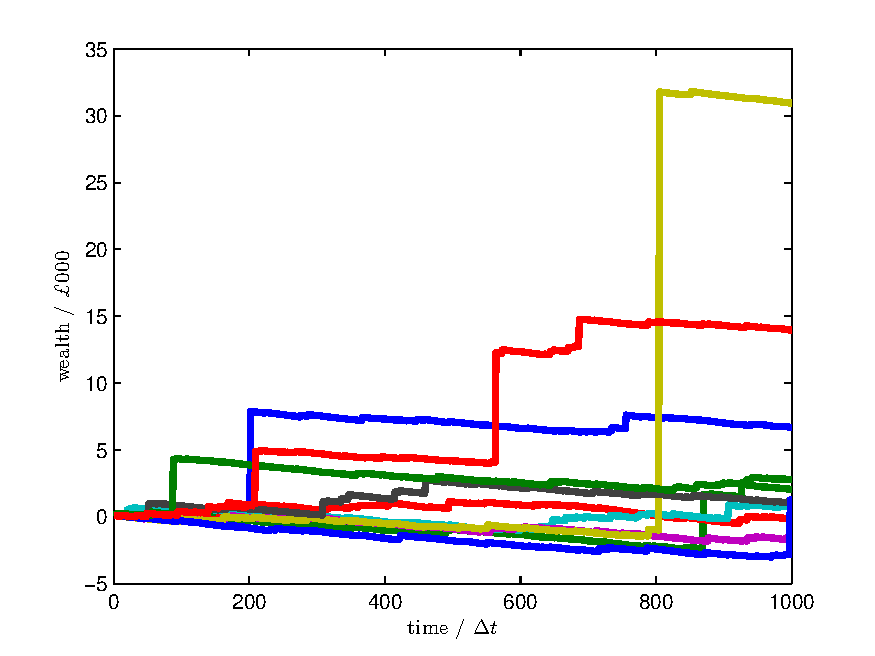
\includegraphics[width=\textwidth]{./chapter_2/figs/lottery_add_traj.pdf}
\caption{Wealth trajectories for the additively repeated St Petersburg lottery, 
with starting wealth, $\x(0)=\$100$, and ticket price, $\F=\$10$. 
Ten trajectories are plotted over 1,000 rounds.\flabel{lottery_add_traj}}
\end{figure}

This implausible conclusion, which does not accord with human behaviour, 
exposes the weakness of judging a gamble by its effect on expected 
wealth. Daniel Bernoulli suggested to resolve the paradox by adopting 
the expected-utility paradigm. His choice of utility function was the 
logarithm, $\gu(\x)=\ln \x$, which, as we now know, produces a decision 
rule equivalent to growth-rate optimisation under multiplicative repetition. 
This correspondence was not appreciated by Bernoulli: indeed, it is unclear 
whether $18^\text{th}$ century mathematics possessed the concepts and 
language required to distinguish between averages over time and across 
systems, even if it had the basic arithmetic tools. In any case, the 
correspondence relies on the choice of a particular utility function, 
and vanishes the moment something other than the logarithm is chosen.

Unfortunately, Bernoulli made a mathematical error in the implementation 
of his own paradigm. This was corrected by Laplace in 
1814~\cite{Laplace1814} and then de-corrected by Menger in 
1934~\cite{Menger1934}, who introduced a further error which led to the 
famous but unjustifiable claim that utility functions must be bounded. We 
will leave this most chequered part of the paradox's history alone -- details, 
including a rebuttal of Menger's analysis, can be found 
in~\cite{PetersGell-Mann2016}. Instead we will focus on what's usually 
presumed Bernoulli meant to write.

\begin{example}{Resolution by logarithmic utility}
Instead of \eref{lottery_ex_wealth}, we calculate the rate of change of expected logarithmic utility,
\bea
\frac{\ave{\d\ln \x}}{\dt} & = & \frac{1}{\dt} \sum_{\gk=1}^\infty \p_\gk \left[\ln(\x+\gD_\gk)-\ln \x\right] \\
&=& \frac{1}{\dt} \sum_{\gk=1}^\infty 2^{-\gk} \ln\left(\frac{\x+\$2^{\gk-1}-\F}{\x}\right), \elabel{lottery_ex_util}
\eea
where $\x$ is the ticket buyer's wealth.

This is finite for all finite ticket prices less than the buyer's wealth plus the smallest 
prize: $\F<\x+\$1$. This can be shown by applying the ratio 
test.\footnotemark\ It may be positive or negative, depending on the values 
of $\F$ and $\x$. \fref{gbar_zero} shows the locus of points in the $(\x,\F)$-plane 
for which the sum is zero.
\end{example}
\footnotetext{The ratio of the $(\gk+1)^\text{th}$ term to the $\gk^\text{th}$ term 
in the sum tends to $1/2$ as $\gk\to\infty$.}
\begin{figure}
\centering
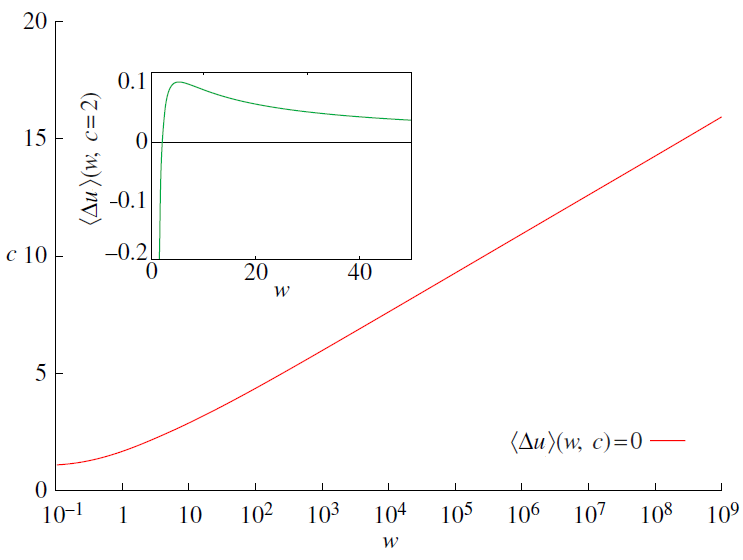
\includegraphics[width=\textwidth]{./chapter_2/figs/gbar_zero.png}
\caption{Locus of points in the $(\x,\F)$-plane for which the expected change in 
logarithmic utility is zero. The inset shows the expected change in utility as a 
function of $\x$ for $\F=\$2$. Adapted from~\cite{Peters2011b}.\flabel{gbar_zero}}
\end{figure}

This resolves the paradox, in that it admits the possibility of the player declining to buy a ticket when his expected change in utility is less than that of the null gamble, \ie zero. Bernoulli argued for this resolution framework in plausible terms, which we have already discussed: the usefulness of a monetary gain depends on how much money you already have. He also argued specifically for the logarithm in plausible terms: the gain in usefulness should be proportional to the fractional gain it represents, $\gd \gu = \d\x/\x$. He did not connect this to the idea of repetition over time. If he had, he might have been less willing to accept Cramer's square-root utility function as an alternative.\footnote{Although there exists a dynamic for which $\gu=\sqrt{\x}$ gives the appropriate stationarity mapping, it is rather more esoteric than the multiplicative repetition with which most of humanity is familiar.}

However, while plausible, the framework relies on a utility function, which must be postulated. It can neither be derived from fundamental considerations nor verified empirically.

Turning to our decision algorithm, we will assume that the lottery is repeated multiplicatively. This means, in effect, that the prizes and ticket price are treated as fractions of the player's wealth, such that the effect of each lottery is to multiply current wealth by a random factor,
\be
\gr_\gk = \frac{\x+\$2^{\gk-1}-\F}{\x}, \quad \p_\gk = 2^{-\gk}.
\ee
This follows precisely our earlier treatment of a gamble with multiplicative dynamics, and we can apply our results directly. 
The time-average (exponential) growth rate is
\be
\gt_\text{m} = \frac{1}{\dt} \lim_{\T\to\infty} \left\{ \frac{1}{\T}  \sum_{\gtau=1}^\T \ln \gr(\gtau) \right\} = \frac{1}{\dt}  \sum_{\gk=1}^\infty 2^{-\gk} \ln \gr_\gk, \elabel{lottery_gbar}
\ee
which is identical to the expression for the rate of change of expected log-utility, 
\eref{lottery_ex_util}. This is, as we've discussed, because $\gt_\text{m}$ is 
the ergodic growth rate for multiplicative dynamics. The result is the same, but 
the interpretation is different: we have assumed less, only that our player is 
interested in the growth rate of his wealth and that he gauges this by imagining 
the outcome of an indefinite sequence of repeated lotteries.

Thus the locus in \fref{gbar_zero} also marks the decision threshold \textit{versus} 
the null gamble under our decision axiom. The player can sensibly decline the 
gamble, even though it results in a divergent change in expected wealth. This 
is illustrated by comparing \fref{lottery_mult_traj}, which shows trajectories of 
multiplicatively repeated lotteries, with the additively repeated lotteries already 
seen in \fref{lottery_add_traj}.
\begin{figure}
\centering
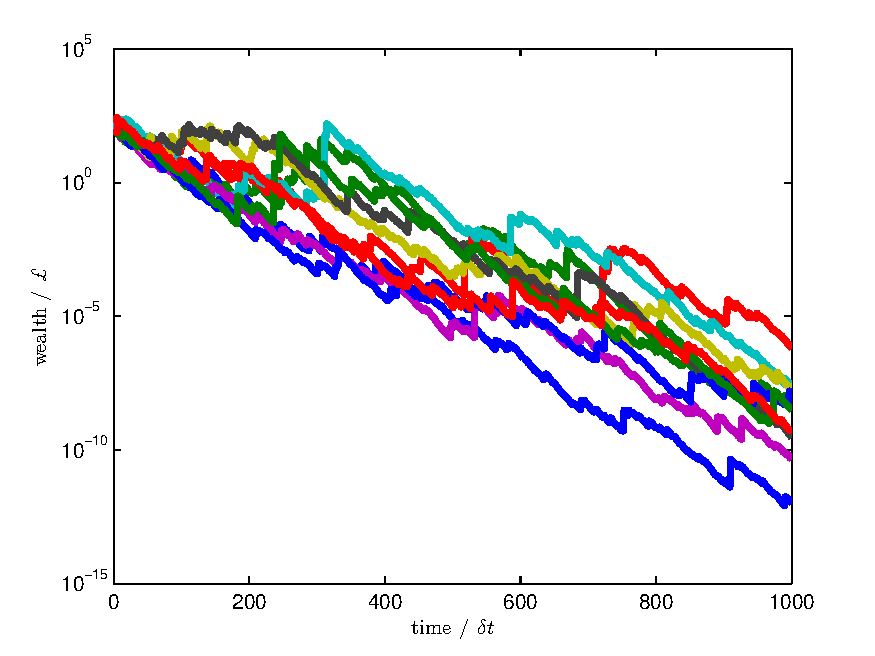
\includegraphics[width=\textwidth]{./chapter_2/figs/lottery_mult_traj.pdf}
\caption{Wealth trajectories for the multiplicatively repeated St Petersburg lottery, 
with starting wealth, $\x(0)=\$100$, and ticket price, $\F=\$10$. Ten 
trajectories are plotted over 1,000 rounds. The realisations of the individual 
lotteries are the same as in \fref{lottery_add_traj} but the mode of repetition is 
different.\flabel{lottery_mult_traj}}
\end{figure}
The trajectories are based on the same sequences of lottery outcomes, only 
the mode of repetition is different. The simulation shows us visually what we 
have already gleaned by analysis: that what appears favourable in the 
expected-wealth paradigm (corresponding to additive repetition) results in a 
disastrous decay of the player's wealth over time under a realistic dynamic.

As $\F\to \x+\$1$ from above in \eref{lottery_gbar}, $\gt_\text{m}$ diverges 
negatively, since the first term in the sum is the logarithm of a quantity approaching 
zero. This corresponds to a lottery which can make the player bankrupt. The effect 
is also shown in the inset of \fref{gbar_zero}.

Treatments based on multiplicative repetition have appeared sporadically in the 
literature, starting with Whitworth in 
1870~\cite[App.~IV]{Whitworth1870}.\footnote{Whitworth was dismissive of early utility theory: ``The result at which we have arrived is not to be classed with 
the arbitrary methods which have been again and again propounded to evade the difficulty of the Petersburg problem\ldots. Formulae have often been proposed, which have possessed the one virtue of presenting a finite result\ldots but they have often had no intelligible basis to rest upon, or\ldots sufficient care has not been taken to draw a distinguishing line between the significance of the result obtained, and the different result arrived at when the mathematical expectation is calculated.'' Sadly he chose to place these revolutionary remarks in an appendix of a college probability textbook.} It is related to the famous Kelly Criterion~\cite{Kelly1956}\footnote{Kelly was similarly unimpressed with the mainstream and noted in his treatment of decision theory, which he developed from the perspective of information theory and which is identical to ergodicity economics with multiplicative dynamics, that the utility function is ``too general to shed any light on the specific problems of communication theory.''}, although Kelly did not explicitly treat the St Petersburg game, and tangentially to \Ito's lemma~\cite{Ito1944}. It appears as an exercise in a well-known text on information theory~\cite[Ex.~6.17]{CoverThomas1991}. Mainstream economics has ignored all this. A full and rigorous resolution of the paradox, including the epistemological significance of the shift from ensemble to time averages, was published recently by one of the present authors~\cite{Peters2011b}.

%%%%%%%%%%%%%%%%%%%%%%%%%%%%%%%%%%%%%%%%%%%%%%%
\subsection{The insurance puzzle}
The insurance contract is an important and ubiquitous type of economic transaction, 
which can be modelled as a gamble. However, it poses a 
puzzle~\cite{PetersAdamou2015b}. In the expected-wealth paradigm, insurance 
contracts shouldn't exist, because buying insurance would only be rational at a 
price at which it would be irrational to sell. More specifically:
\begin{enumerate}
\item To be viable, an insurer must charge an insurance premium of at least the 
expectation value of any claims that may be made against it, called the ``net 
premium'' \cite[p.~1]{KaasETAL2008}.
\item The insurance buyer therefore has to be willing to pay more than the net 
premium so that an insurance contract may be successfully signed.
\item Under the expected-wealth paradigm it is irrational to pay more than the 
net premium, and therefore insurance contracts should not exist.
\end{enumerate}
In this picture, an insurance contract can only ever be beneficial to one party. It 
has the anti-symmetric property that the expectation value of one party's gain is 
the expectation value of the other party's loss.

The puzzle is that insurance contracts are observed to exist.\footnote{Something 
of an understatement. The Bank for International Settlements estimated the 
market value of all the world's derivatives contracts, which are essentially 
insurance contracts, as \$15 trillion in the first half of 2015 (see 
\url{http://www.bis.org/statistics/d5\_1.pdf}). That's six times the gross domestic 
product of the United Kingdom.} Why? Classical resolutions appeal to utility 
theory (\ie psychology) and asymmetric information (\ie deception). However, 
our decision theory naturally predicts contracts with a range of prices that 
increase the time-average growth rate for both buyer and seller. We illustrate 
this with an example drawn from maritime trade, in which the use of insurance 
has a very long history.\footnote{Contracts between Babylonian traders and 
lenders were recorded around 1750 BC in the Code of Hammurabi. Chinese 
traders practised diversification by spreading cargoes across multiple vessels 
even earlier than this, in the third millennium BC.} A similar 
example was used by Bernoulli~\cite{Bernoulli1738}.

\begin{example}{A shipping contract}
We imagine a shipowner sending a cargo from St Petersburg to Amsterdam, with the following parameters:
\begin{itemize}
\item owner's wealth, $\x_\text{own}=\$100,000$;
\item gain on safe arrival of cargo, $\G=\$4,000$;
\item probability ship will be lost, $\p=0.05$;
\item replacement cost of the ship, $\C=\$30,000$; and
\item voyage time, $\dt=1$ month.
\end{itemize}
An insurer with wealth $\x_\text{ins}=\$1,000,000$ proposes to insure the voyage for a 
fee, $\F=\$1,800$. If the ship is lost, the insurer pays the owner $\gL=\G+\C$ to make him 
good on the loss of his ship and the profit he would have made.
\end{example}
We phrase the decision the owner is facing as a choice between 
two gambles. 

\begin{definition}{The owner's gambles}

Sending the ship uninsured corresponds to gamble o1
\bea
\gD_1^{(\text{o1})} = \G, &\quad& \p_1^{(\text{o1})} = 1-p;\\
\gD_2^{(\text{o1})} = -\C, &\quad& \p_2^{(\text{o1})} = p.
\eea
Sending the ship fully insured corresponds to gamble o2
\bea
\gD_1^{(\text{o2})} = \G-\F &\quad& \p_1^{(\text{o2})} = 1.
\eea
This is a trivial ``gamble'' because all risk has been 
transferred to the insurer. 
\end{definition}

We also model the insurer's decision whether to offer the contract as
a choice between two gambles

\begin{definition}{The insurer's gambles}

Not insuring the ship corresponds to gamble i1, which is the null gamble
\bea
\gD_1^{(\text{i1})} = 0 &\quad& \p_1^{(\text{i1})} = 1.
\eea

Insuring the ship corresponds to gamble i2
\bea
\gD_1^{(\text{i2})} = +\F, &\quad& \p_1^{(\text{i2})} = 1-p;\\
\gD_2^{(\text{i2})} = -\gL+\F, &\quad& \p_2^{(\text{i2})} = p.
\eea
\end{definition}

We ask whether the owner should sign the contract, and whether the insurer should have proposed it.

\begin{example}{Expected-wealth paradigm}
In the expected-wealth paradigm (corresponding to additive repetition under 
the time paradigm) decision makers
maximise the rate of change of the expectation values of their wealths, according to \eref{ex_crit}:
Under this paradigm the owner collapses gamble o1 into the scalar

\bea
\gt_a^{(\text{o1})} &=& \frac{\ave{\d\x}}{\dt}\\
&=&\frac{\ave{\gD^{(\text{o1})}}}{\dt}\\
&=&\frac{(1-p) \G + p (-\C) }{\dt}\\
&=&\$ 2,300\text{ per month,}
\eea

and gamble o2 into the scalar

\bea
\gt_a^{\text{o2}} &=&\frac{\ave{\gD^{(\text{o2})}}}{\dt}\\
&=&\frac{(\G-\F) }{\dt}\\
&=&\$2,200 \text{ per month.}
\eea
The difference, $\delta\gt_a^\text{o}$,  between the expected rates 
of change in wealth with and without a signed contract is the expected 
loss minus the fee per round trip,
\be
\delta\gt_a^\text{o}=\gt_a^{\text{o2}}-\gt_a^{\text{o1}}= \frac{\p \gL - \F}{\dt}.
\elabel{dro}
\ee
The sign of this difference indicates whether the insurance contract is beneficial
to the owner. In the example this is not the case, $\delta\gt_a^\text{o}=-\$100$ per month.

The insurer evaluates the gambles i1 and i2 similarly, with the result
\be
\gt_a^{(\text{i1})}  = \$0 \text{ per month,}
\ee
and
\bea
\gt_a^{(\text{i2})}  &=& \frac{\F-\p \gL}{\dt} \elabel{r}\\ 
&=& \$100 \text{ per month.}
\eea
Again we compute the difference -- the net benefit to the insurer that arises from signing the contract
\be
\delta\gt_a^\text{i}=\gt_a^{\text{i2}}-\gt_a^{\text{i1}}= \frac{\F- \p \gL}{\dt}.
\elabel{dri}
\ee
In the example this is $\delta\gt_a^\text{i}=\$100$ per month, meaning that in the 
world of the expected-wealth paradigm the insurer will offer the contract.
\end{example}

Because only one party (the insurer) is willing to sign, no contract will come into existence. We could think that we got
the price wrong, and the contract would be sigend if offered at a different fee. 
But this is not the case, and that's the fundamental insurance puzzle: in the
world created by expected-wealth maximisation no price exists at which both
parties will sign the contract.

Looking at \eref{dro} and \eref{dri} we notice the anti-symmetric relationship between
the two expressions,  
$\delta\gt_a^\text{o}=-\delta\gt_a^\text{i}$.
By symmetry, there can be no fee at which both expressions are positive. 
Hence there are no circumstances in the world created by the 
expected-wealth paradigm under which both parties will sign. Insurance
contracts cannot exist in this world.

One party winning at the expense of the other makes insurance an 
unsavoury business in the expected-wealth paradigm. This is further 
illustrated in \fref{ins_lin}, which shows the change in the rate of 
change of expected wealth (the decision variable) for both parties 
as a function of the fee, $\F$.
\begin{figure}
\centering
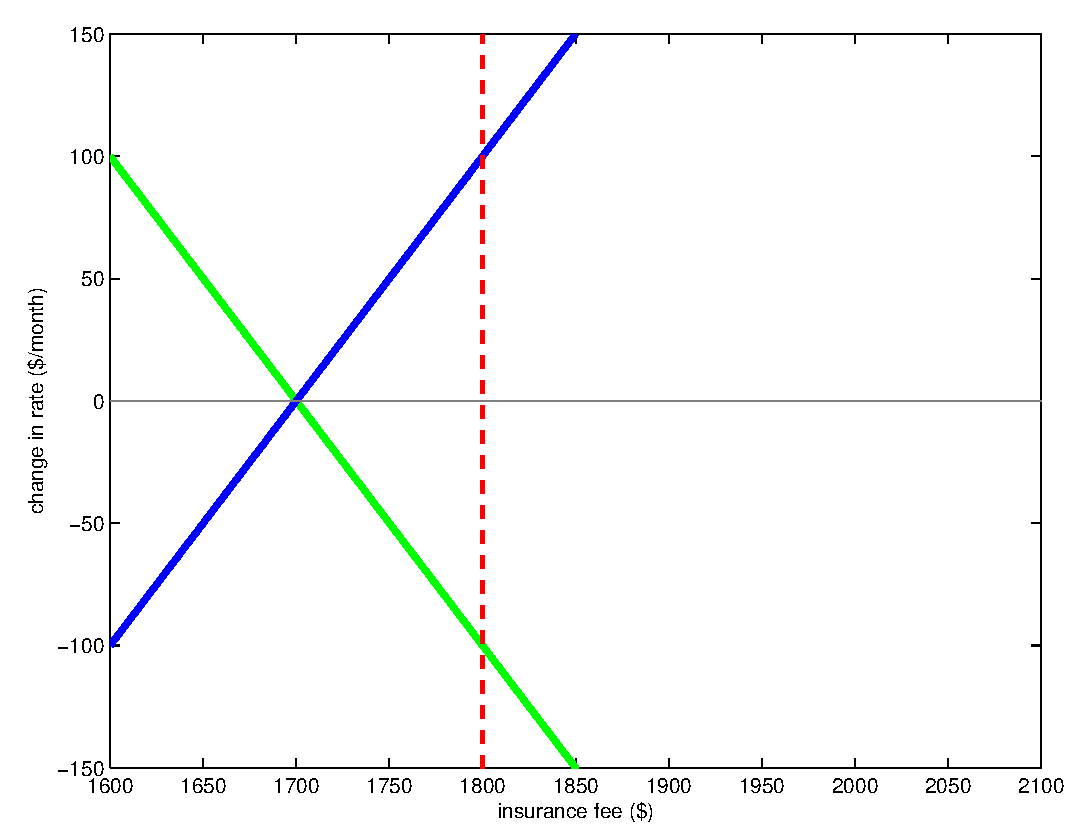
\includegraphics[width=\textwidth]{./chapter_2/figs/ins_lin_cropped.pdf}
\caption{Change in the rate of change of expected wealth for the shipowner (green) and the 
insurer (blue) as a function of the insurance fee, $\F$.\flabel{ins_lin}}
\end{figure}
There is no price at which the decision variable is positive for the both parties. The best they can 
do is to pick the price at which neither of them cares whether they sign or not.

In this picture, the existence of insurance contracts requires some asymmetry between the contracting parties, such as:
\begin{itemize}
\item different attitudes to bearing risk;
\item different access to information about the voyage;
\item different assessments of the riskiness of the voyage;
\item one party to deceive, coerce, or gull the other into a bad decision.
\end{itemize}
It is difficult to believe that this is truly the basis for a market of the size and global reach of the insurance market.

\subsubsection{Solution in the time paradigm}

\begin{example}{Time paradigm}
The insurance puzzle is resolved in the `time paradigm', \ie using 
the growth-optimal decision theory we have developed in this lecture
and multiplicative repetition. Again, we pause to reflect what multiplicative
repetition means compared to additive repetition. This is important because
additive repetition is equivalent to the expected-wealth paradigm that 
created the insurance puzzle.  Multiplicative repetition means that the 
ship owner sends out a ship and a cargo whose values are proportional to 
his wealth at the start of each voyage. A rich owner who has had many 
successful voyages will send out more cargo, a larger ship, or perhaps a \textit{flotilla}, while an owner 
to whom the sea has been a cruel mistress will send out a small vessel until his luck changes.
Under additive repetition, the ship owner would send out the same amount
of cargo on each journey, irrespective of his wealth. Shipping companies
of the size of Evergreen or Maersk would be inconceivable under additive repetition,
where returns on successful investments are not reinvested.

The two parties seek to maximise
\be
\gt_m = \lim_{\Dt\to\infty}\frac{\D\gv(\x)}{\Dt} = \frac{\ave{\d\ln \x}}{\dt},
\ee
where we have used the ergodic property of $\D\gv(\x)=\D\ln\x$
under multiplicative repetition.

The owner's time-average growth rate without insurance is 
\be
\gt_m^\text{o1} = \frac{(1-\p)\ln(\x_\text{own}+\G)+\p\ln(\x_\text{own}-\C) - \ln(\x_\text{own})}{\dt}
\ee
or 1.9\% per month. 
His time-average growth rate with insurance is 
\be
\gt_m^\text{o2} = \frac{\ln(\x_\text{own}+\G-\F)-\ln(\x_\text{own})}{\dt}
\ee
or 2.2\% per month. This gives a net benefit for the owner of
\be
\d\gt_m^o = \gt_m^\text{o1}-\gt_m^\text{o2} \approx +0.24\% \text{ per month.} 
\ee
The time paradigm thus creates a world where the owner will sign the contract.

What about the insurer? Without insurance, the insurer plays the null gamble, and
\be
\gt_m^{\text{i1}}= \frac{0}{\dt}
\ee
or 0\% per month. His time-average growth rate with insurance is 
\be
\gt_m^{\text{i2}} = \frac{(1-p)\ln(\x_\text{ins}+\F) + p\ln(\x_\text{ins}+\F-\gL) - \ln(\x_\text{ins})}{\dt}
\ee
or 0.0071\% per month. The net benefit to the insurer is therefore also
\be
\delta\gbar_m^{\text{i}} = \gt_m^{\text{i2}}-\gt_m^{\text{i1}}
\ee
\ie 0.0071\% per month. Unlike the expected wealth paradigm, the time paradigm with multiplicative repetition 
creates a world where an insurance contract can exist -- there exists a range of fees $\F$ at which
both parties gain from signing the contract! 
\end{example}


We view this as the
\begin{keypts}{Fundamental resolution of the insurance puzzle:}
The buyer and seller of an insurance contract both sign when it increases the time-average growth rates of their wealths.
\end{keypts}
It requires no appeal to arbitrary utility functions or asymmetric circumstances, rather it arises naturally from the model of human decision-making that we have set out. \fref{ins_log} shows the mutually beneficial range of insurance fees predicted by our model.
\begin{figure}
\centering
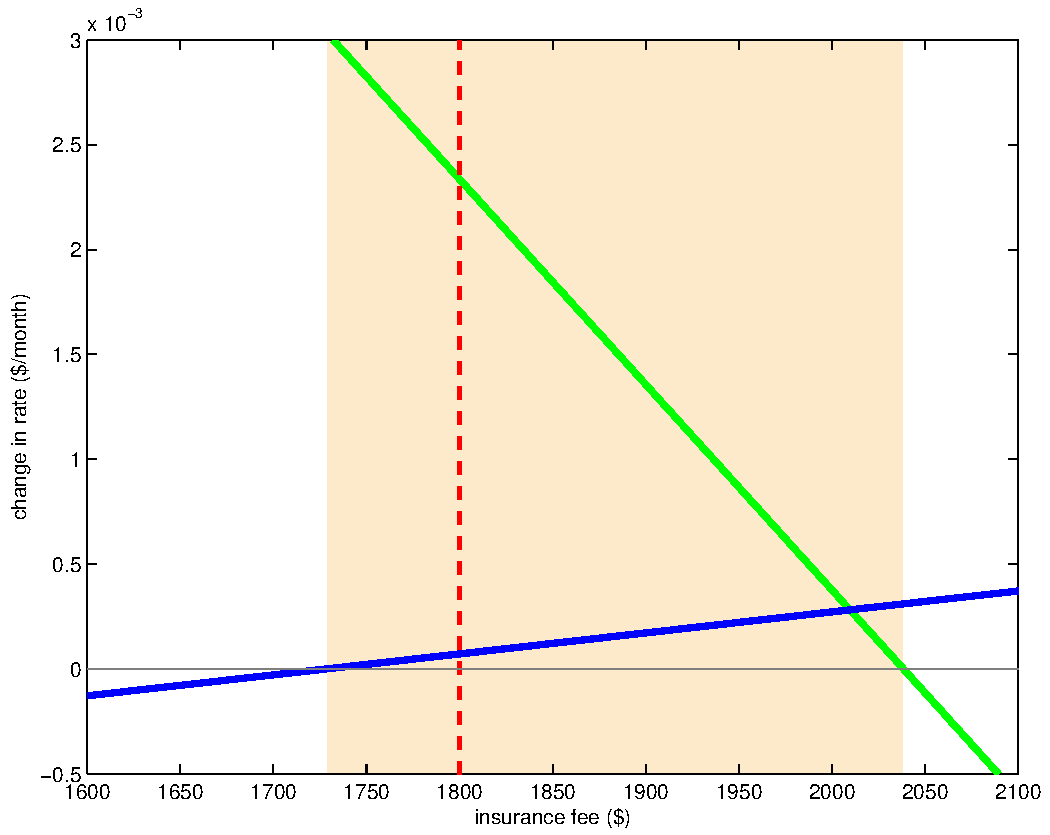
\includegraphics[width=\textwidth]{./chapter_2/figs/ins_log_cropped.pdf}
\caption{Change in the time-average growth rate of wealth for the shipowner (green) and the insurer (blue) as a function of the insurance fee, $F$. The mutually beneficial fee range is marked by the beige background.\flabel{ins_log}}
\end{figure}
Generalizing, the message of the time paradigm is that business happens when both parties gain.
In the world created by this model any agreement, any contract, any commercial interaction 
comes into existence because it is mutually beneficial.

%\printglossary[title=Glossary,type=\acronymtype]
%%
%\printglossary[title=List of Symbols]
\subsubsection{The classical solution of the insurance puzzle}
\seclabel{The classical solution of the insurance puzzle}

%\begin{example}{Expected-utility paradigm}
%Let's look at the solution in the expected-utility paradigm. Our players now seek to maximise the rate of change of their expected utility,
%\be
%\ave{r_u} \equiv \frac{\ave{\Du(W)}}{\Dt}.
%\ee
%To make the example concrete, we will use $u(W)=\sqrt{W}$, as suggested by Cramer~\cite{Cramer1728}, for both parties.
%
%The owner has
%\be
%\ave{r_u}_\text{own}^\text{un} = \frac{(1-p)u(W_\text{own}+G)+pu(W_\text{own}-C) - u(W_\text{own})}{\Dt}
%\ee
%or 3.37 `utils'\footnotemark\ per month without insurance, and 
%\be
%\ave{r_u}_\text{own}^\text{in} = \frac{u(W_\text{own}+G-F)-u(W_\text{own})}{\Dt}
%\ee
%or 3.46 utils per month with insurance. The change in $\ave{r_u}_\text{own}$ is 
%\be
%\delta\ave{r_u}_\text{own} = \ave{r_u}_\text{own}^\text{in} - \ave{r_u}_\text{own}^\text{un},
%\ee
%\ie 0.094 utils per month, and the owner should sign.
%
%The contract is also favourable from the insurer's perspective. If he does no business, then 
%\be
%\ave{r_u}_\text{ins}^\text{un} = \frac{0}{\Dt}
%\ee
%or zero utils per month. If he extends insurance, then
%\be
%\ave{r_u}_\text{ins}^\text{in} = \frac{(1-p)u(W_\text{ins}+F) + pu(W_\text{ins}+F-L) - u(W_\text{ins})}{\Dt}
%\ee
%or 0.043 utils per month and his change in $\ave{r_u}_\text{ins}$ is positive:
%\be
%\quad \delta\ave{r_u}_\text{ins} = \ave{r_u}_\text{ins}^\text{in} - \ave{r_u}_\text{ins}^\text{un},
%\ee
%\ie 0.043 utils per month.
%\end{example}
%\footnotetext{The general unit of utility. Here $1\,\text{util} = \sqrt{\$}\,1$, whatever that might mean.}
The classical solution of the insurance puzzle is identical to the classical solution of the St Petersburg paradox.
Wealth is replaced by a non-linear utility function of wealth, which breaks the symmetry of the 
expected-wealth paradigm. While it is always true that $\delta\ave{r}_\text{own}=-\delta\ave{r}_\text{ins}$, 
the expected growth rates of non-linear utility functions don't share this anti-symmetry. A difference in 
the decision makers' wealths is sufficient, though often different utility functions are assumed for owner and insurer, 
which is a model that can create pretty much any behavior. The downside of a model with this ability is, of course, 
that it makes no predictions -- nothing is ruled out, so the model cannot be falsified.
%
%This represents the classical resolution of the insurance puzzle. The symmetry broken by the different wealths $W_\text{own}$ and $W_\text{ins}$, which now appear in $\ave{r_u}$ since the utility function is nonlinear.\footnote{Note that the symmetry could also have been broken by assigning different utility functions to the two parties, even if their wealths were the same. However, it suffices only that their wealths be different for the puzzle to be resolved.} Certain combinations of $W_\text{own}$, $W_\text{ins}$, and $u$ will admit a range of mutually beneficial prices, $F$. This is visible as the beige region in \fref{ins_sqrt}, which plots the decision variable, $\delta\ave{r_u}$, for both parties as a function of the fee, $F$.
%\begin{figure}
%\centering
%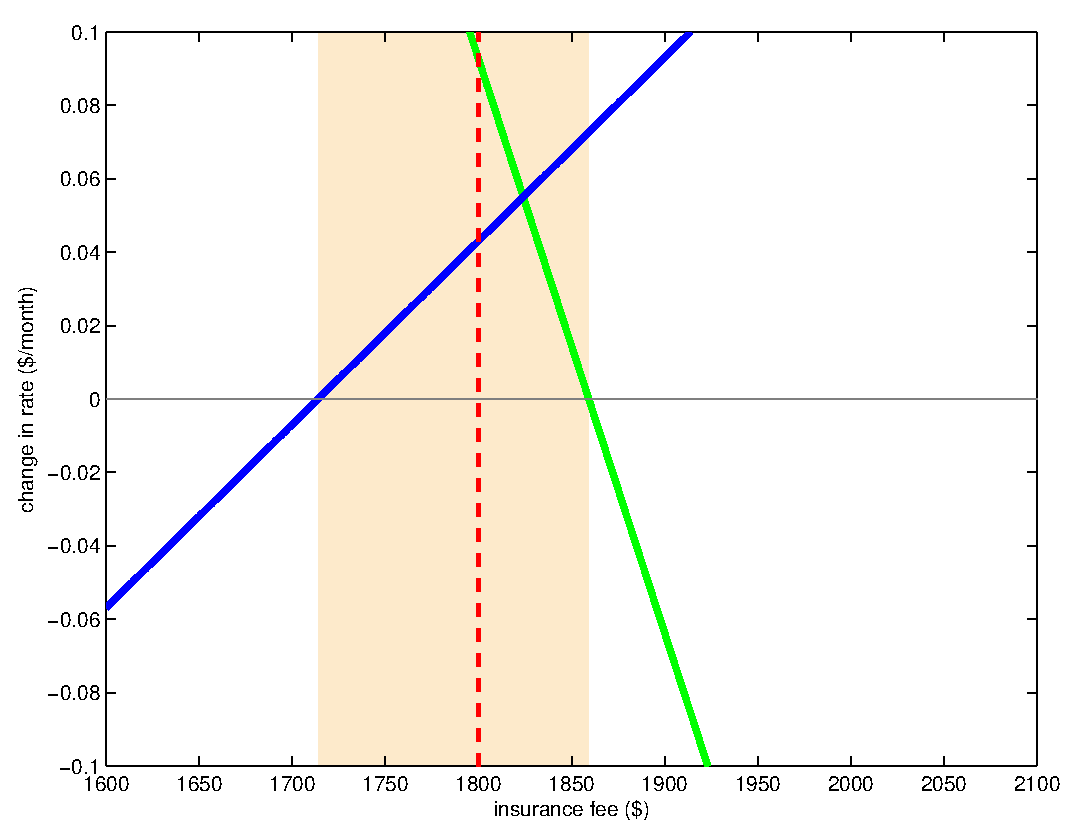
\includegraphics[width=\textwidth]{./chapter_2/figs/ins_sqrt_cropped.pdf}
%\caption{Change in the rate of change of expected square-root utility for the shipowner (green) and the insurer (blue) as a function of the insurance fee, $F$. The mutually beneficial fee range is marked by the beige background.\flabel{ins_sqrt}}
%\end{figure}
%Utility theory does not rule out insurance contracts -- it is {\it possible} to create a win-win deal -- but does not rule them in either. Furthermore, invoking arbitrary and unobservable utility functions hardly seems a satisfying resolution of the puzzle.